% SCAI 2026 - 2-page Extended Abstract
% Using LLNCS Springer template
%
\documentclass[runningheads]{llncs}
%
\usepackage[T1]{fontenc}
\usepackage{graphicx}
\usepackage{hyperref}
\usepackage{color}
\usepackage{booktabs}
\usepackage{multirow}
\usepackage{enumitem}
 \usepackage{amsmath}
\renewcommand\UrlFont{\color{blue}\rmfamily}
\urlstyle{rm}

\usepackage{caption}
\captionsetup{font=tiny}

% ============================================================================
% BENCHMARK RESULTS - From benchmark_results.json and TrOCR predictions
% ============================================================================
\newcommand{\ctcCER}{12.24}      % From benchmark_results.json (ctc_simple)
\newcommand{\ctcWER}{37.35}      % From benchmark_results.json (ctc_simple)

\newcommand{\ctcCacc}{87.72}


% TrOCR variants from benchmark
\newcommand{\trocrBestCER}{8.55}     % trocr_smi_synth - best accuracy
\newcommand{\trocrBestWER}{28.16}    % trocr_smi_synth

\newcommand{\trocrBestCacc}{91.56}

% Translation metrics from end-to-end pipeline evaluation (ctc_simple)
\newcommand{\bleuScore}{10.40}
\newcommand{\chrfScore}{33.85}
\newcommand{\terScore}{76.30}

% Model size from checkpoint file
\newcommand{\modelSize}{23MB}

\newcommand{\benchmarkSamples}{1048}  % Total benchmark samples (1000 HF + 48 book)
\newcommand{\hfTestSamples}{1000}    % Språkbanken HF test subset
\newcommand{\bookTestSamples}{48}    % Historical book samples


\newcommand{\trocrSmiNorPredSynthCER}{17.46}  % trocr_smi_nor_pred_synth
\newcommand{\trocrSmiNorPredSynthWER}{48.20}
\newcommand{\trocrSmiPredSynthCER}{15.85}  % trocr_smi_pred_synth
\newcommand{\trocrSmiPredSynthWER}{45.76}
\newcommand{\trocrSmiSynthCER}{8.55}  % trocr_smi_synth
\newcommand{\trocrSmiSynthWER}{28.16}

\newcommand{\trocrSmiNorPredCER}{26.97}  % trocr_smi_nor_pred
\newcommand{\trocrSmiNorPredWER}{64.84}
\newcommand{\trocrSmiPredCER}{25.30}  % trocr_smi_pred
\newcommand{\trocrSmiPredWER}{63.61}
\newcommand{\trocrSmiNorCER}{26.22}  % trocr_smi_nor
\newcommand{\trocrSmiNorWER}{67.08}
\newcommand{\trocrSmiCER}{24.12}  % trocr_smi
\newcommand{\trocrSmiWER}{63.50}


% Timing, size, and efficiency
\newcommand{\trocrSize}{350MB}
\newcommand{\trocrBestTime}{12.41}
\newcommand{\ctcTime}{0.033}
\newcommand{\speedupFactor}{380}
\newcommand{\sizeRatio}{15}
\newcommand{\cerAccGap}{3.84}

% Word and character accuracy (table columns)
\newcommand{\trocrBestWordAcc}{72.49}
\newcommand{\ctcWordAcc}{62.45}
\newcommand{\trocrPredSynthCharAcc}{84.15}
\newcommand{\trocrPredSynthWordAcc}{54.24}
\newcommand{\trocrPredSynthTime}{12.08}
\newcommand{\trocrSmiCharAcc}{75.88}
\newcommand{\trocrSmiWordAcc}{36.50}
\newcommand{\trocrSmiTime}{16.23}

% \newcommand{\ctcSimpleCER}{12.24}  % ctc_simple
% \newcommand{\ctcSimpleWER}{37.35}

%
\begin{document}
%
\title{OCR and Machine Translation Pipeline for Low-Resource S\'{a}mi Languages}
%
%\titlerunning{OCR and MT for S\'{a}mi Languages}
%
\vspace{-0.9cm}
\author{Jan Musiol\inst{1} \and
Aparna S. Varde\inst{2} \and
Juan Heredia\inst{3}}
%
\institute{University of Southern Denmark (1. Sondenborg, 2. Vejle, 3. Odense), Denmark\\
\email{jamus23@student.sdu.dk, \{apva, jehm\}@mmmi.sdu.dk}}

\maketitle

\vspace{-0.7cm}
%
\begin{abstract}
Northern S\'{a}mi is a low-resource language with Optical Character Recognition (OCR) challenges, e.g. limited training data \& diacritical characters.
In this work, we propose a 2-phase pipeline of OCR \& machine translation (MT) comprising lightweight Convolutional Neural Network (CNN) \& Connectionist Temporal Classification (CTC) architecture. We compare this to pre-trained Transformer OCR (TrOCR) models from National Library of Norway.
% While the best TrOCR ($\sim$350MB) model has \trocrBestCER\% Character Error Rate (CER), our CNN-CTC model outperforms this baseline with \ctcCER\% CER on \benchmarkSamples{} samples while requiring only \modelSize{} , making it practical for resource-constrained deployment. Performance degrades for sentences of 20+ words.
The best TrOCR ($\sim$350MB) model gets \trocrBestCacc\% character accuracy. Our CNN-CTC model follows this with \ctcCacc\% accuracy on \benchmarkSamples{} samples, needing only \modelSize{}, and is thus practical for resource-constrained deployment. %Performance degrades for sentences of 20+ words.
End-to-end evaluation on \bookTestSamples{} parallel sentences reveals viable OCR in our model. %, though with limited MT quality.
\vspace{-0.2cm}

\keywords{OCR \and MT \and
Low-Resource Languages \and S\'{a}mi \and DL \and CTC}
\end{abstract}
%
% ============================================================================
% SECTION 1: INTRODUCTION (~0.5 page)
% ============================================================================
\vspace{-1cm}
\section{Introduction}
\vspace{-0.2cm}
S\'{a}mi languages are endangered groups of Uralic languages spoken by indigenous people in northern Norway, Sweden, Finland \& Russia. 
Northern S\'{a}mi is most widely-spoken ($\sim$25,000 speakers). Yet many historical texts are at risk due to lack of digitization \& OCR challenges, especially special diacritical characters (\'{A}/\'{a}, \v{C}/\v{c}, {\DJ}/{\dj}, {\NG}/{\ng}, \v{S}/\v{s}, {\TH}/{\th}, \v{Z}/\v{z}, e.g. Fig.~\ref{fig:example}). Most OCR research focuses on high-resource languages, leaving S\'{a}mi underrepresented. Commercial systems perform poorly on S\'{a}mi orthography~\cite{ref_sprakbanken}. Transformer models e.g. TrOCR
~\cite{ref_trocr,ref_sprakbanken}
from National Library of Norway do well (\trocrBestCER\% CER) but need \trocrSize{}+, limiting deployment in resource-constrained environment.

% \begin{figure}[h]
% \centering
% 
\includegraphics[width=0.85\textwidth]{figures/sami_alphabet_cut.png}
% \caption{Northern S\'{a}mi special characters with example words.}
% \label{fig:alphabet}
% \end{figure}

\vspace{-0.5cm}
\begin{figure}[h]
\centering
\vspace{-0.3cm}
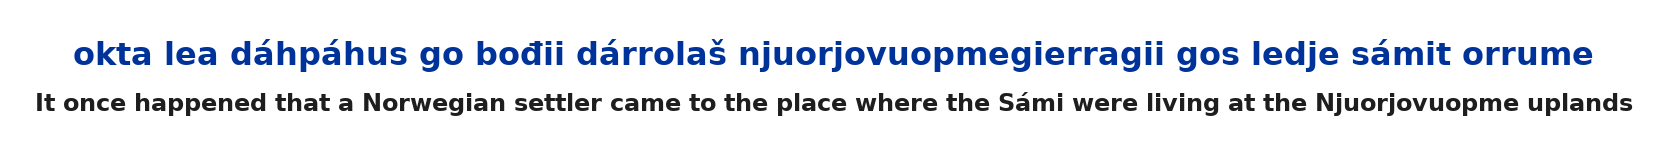
\includegraphics[width=0.9\textwidth]{figures/entry_80.png}
\footnotesize
\vspace{-0.3cm}
\caption{Example sentence from Johan Turi's ``Muitalus s\'{a}miid birra''~\cite{ref_turi} with translation.}
% "\textit{It once happened that a Norwegian settler came to the place where the Sámi were living at the Njuorjovuopme uplands.}"
\label{fig:example}
\end{figure}
\vspace{-0.7cm}
\normalsize

We propose a novel solution of {\it CNN-CTC for S\'{a}mi}, with comparative study on sentence-length accuracy etc. It is motivated by related work, e.g. \cite{corallo2023optical}. 

% ============================================================================
% SECTION 2: METHOD (~0.75 page)
% ============================================================================
\vspace{-0.5cm}
\section{Methodology, Data and Architecture}
\vspace{-0.2cm}
In our proposed {\it CNN-CTC for S\'{a}mi} model, we use the Spr\r{a}kbanken synthetic S\'{a}mi OCR data~\cite{ref_sprakbanken} for training. Evaluation occurs with 2 distinct sets: \textbf{a)} Spr\r{a}kbanken validation split (\hfTestSamples{} synthetic line images) for OCR benchmarking; \textbf{b)} \bookTestSamples{} parallel handpicked Northern S\'{a}mi--English sentence pairs in Johan Turi's ``Muitalus s\'{a}miid birra''~\cite{ref_turi}.
Our CNN-CTC system architecture~\cite{ref_crnn} has
7-layer CNN, bidirectional LSTM encoder (256 units), CTC decoder 32×800px inputs, trained on 276k samples with 395-character vocabulary. VGG-16/19, ResNet-50 backbones fail to converge, and uses CTC loss.
The proposed pipeline thus offers a CLI tool to specify images and select an OCR model. It runs translation of TartuNLP neural MT API~\cite{ref_tartunlp}, on completion returning benchmark data in metrics: CER, WER (OCR); BLEU,
chrF,
TER (MT).

% We trained a CNN-CTC architecture~\cite{ref_crnn} using CTC loss~\cite{ref_ctc}:
% \textbf{ctc\_simple} is a 7-layer CNN (64$\rightarrow$128$\rightarrow$256$^2$$\rightarrow$512$^3$ channels, batch norm on layers 4--5), bidirectional LSTM encoder (256 units), CTC decoder, 32$\times$800px input.
% Training used AdamW (lr=$10^{-4}$, 100 epochs, batch 32, early stopping) on 276k samples with 395-character vocabulary.
% ============================================================================
% SECTION 3: RESULTS & DISCUSSION (~0.5 page)
% ============================================================================
\vspace{-0.6cm}
\section{Results and Discussion}

% Table with Error rates
% Table~\ref{tab:results} compares TrOCR variants and our CNN-CTC model on the \benchmarkSamples-sample benchmark.
% \begin{table}[h]
% \centering
% \caption{OCR benchmark on 1013 samples. Lower CER/WER is better.}
% \label{tab:results}
% \small
% \begin{tabular}{@{}lccccc@{}}
% \toprule
% Model & Type & CER (\%) & WER (\%) & s/img & Size \\
% \midrule
% trocr\_smi\_synth$^*$ & Transf. & \textbf{8.44} & \textbf{27.51} & 15.16 & 350MB \\
% \textbf{ctc\_simple (ours)} & CNN & 12.28 & 37.55 & \textbf{0.04} & 23MB \\
% trocr\_smi\_pred\_synth$^*$ & Transf. & 16.07 & 45.83 & 13.27 & 350MB \\
% trocr\_smi & Transf. & 24.44 & 63.84 & 29.30 & 350MB \\
% \bottomrule
% \end{tabular}

% {\footnotesize $^*$\texttt{smi}=S\'{a}mi data, \texttt{pred}=+auto-transcribed, \texttt{synth}=+synthetic pre-training.}
% \end{table}

% Table with accuracy rates
\vspace{-0.3cm}
Table~\ref{tab:results} compares TrOCR variants and our CNN-CTC model on the benchmark. % \benchmarkSamples-sample benchmark.
The best transformer (trocr\_smi\_synth) reaches \trocrBestCacc\% character accuracy but requires $\sim$\trocrSize{} and \trocrBestTime{}s per image. Our ctc\_simple trails it by \cerAccGap{} accuracy points while being roughly \sizeRatio$\times$ smaller and \speedupFactor$\times$ faster, a favourable trade-off for resource-constrained environment. 
\vspace{-0.5cm}

\vspace{-0.5cm}

\begin{table}[h]
\centering
\tiny
% \caption{OCR benchmark on 1013 samples. Higher Char./Word Acc.\ is better. Character Accuracy is computed as $100 - \text{CER}$ and Word Accuracy as $100 - \text{WER}$, where CER (Character Error Rate) and WER (Word Error Rate) are normalized Levenshtein edit distances at the character and word level, respectively.}

\caption{OCR benchmark on \benchmarkSamples{} samples.}
\label{tab:results}
\begin{tabular}{@{}lccccc@{}}
\toprule
Model & Type & Char.\ Acc.\ (\%) & Word Acc.\ (\%) & s/img & Size \\
\midrule
trocr\_smi\_synth$^*$ & Transf. & \textbf{\trocrBestCacc} & \textbf{\trocrBestWordAcc} & \trocrBestTime & \trocrSize \\
\textbf{ctc\_simple (ours)} & CNN & \ctcCacc & \ctcWordAcc & \textbf{\ctcTime} & \textbf{\modelSize} \\
trocr\_smi\_pred\_synth$^*$ & Transf. & \trocrPredSynthCharAcc & \trocrPredSynthWordAcc & \trocrPredSynthTime & \trocrSize \\
trocr\_smi & Transf. & \trocrSmiCharAcc & \trocrSmiWordAcc & \trocrSmiTime & \trocrSize \\
\bottomrule
\end{tabular}
\\[2pt]
Char./Word Acc.\ = $100 - $ CER/WER (normalized Levenshtein). \\
$^*$\texttt{smi}=S\'{a}mi data, \texttt{pred}=+auto-transcribed, \texttt{synth}=+synthetic pre-training.
% $^*$\texttt{smi}=S\'{a}mi data, \texttt{pred}=+auto-transcribed, \texttt{synth}=+synthetic pre-training.
\end{table}

% \vspace{-0.4cm}
\begin{figure}[t]
\centering
\vspace{-0.3cm}

\includegraphics[width=0.5\textwidth]{figures/sentence_length_analysis.png}
\vspace{-0.2cm}
\tiny
\caption{Character accuracy v. sentence length}
\vspace{-0.5cm}
\label{fig:length}
\end{figure}
\normalsize
\vspace{-0.5cm}

\textbf{Sentence Length.}
Fig.~\ref{fig:length} shows that character accuracy is stable (mean $\sim$88\%, median $>$95\%) for sentences up to $\sim$30 words and drops sharply ($\sim$50\% mean) for longer sentences ($n=7$ in this bin). We attribute this to horizontal compression at the fixed 32$\times$800px input resolution.

\textbf{End-to-End Pipeline.}
On \bookTestSamples{} parallel sentence pairs, a full OCR(ctc\_simple) $\rightarrow$ MT pipeline yields BLEU \bleuScore, chrF \chrfScore, and TER \terScore. While 62.5\% of inputs achieve a perfect normalized match (after removing punctuation and collapsing whitespace), overall translation quality remains limited (BLEU $\sim$10), indicating that MT quality is the primary constraint on end-to-end performance, though OCR errors ($\sim$88\% avg.\ character accuracy on the book subset) contribute to pipeline limitations.



% ============================================================================
% SECTION 4: CONCLUSION
% ============================================================================
% \section{Conclusion and Future Work}
% This work offers a solution for digitizing S\'{a}mi corpora. Providing a choice between OCR approaches: a transformer model (8.44\% CER, 350MB, 15s/img) when accuracy is paramount, or our CNN-CTC model (12.28\% CER, 23MB, 0.04s/img) when footprint and speed matter---giving up 3.84 CER points for a roughly 15$\times$ smaller and 420$\times$ faster system that trains on modest hardware. End-to-end results further indicate that translation quality, rather than OCR accuracy alone, is the primary performance bottleneck of the full pipeline.
% Future iterations will address the current constraints of our pipeline. We plan to expand the training corpus beyond synthetic data to include real-world samples, bridging the domain gap, and to integrate automated layout analysis, removing the reliance on pre-segmented text lines.
% Code: \url{https://github.com/magwrap/sami-ocr-translate} (made public upon publication).

\vspace{-0.5cm}
\section{Conclusion and Future Work}
\vspace{-0.2cm}
Our work in this paper offers a solution for digitizing S\'{a}mi corpora, with 2 OCR options:
{\bf 1. Transformer} (\trocrBestCacc\% char.\ accuracy, \trocrSize{}, \trocrBestTime{}s/img): if accuracy is paramount.
{\bf 2. CNN-CTC} (\ctcCacc\% char.\ accuracy, \modelSize{}, \ctcTime{}s/img): if footprint and speed matter, giving \cerAccGap{} accuracy points for a $\sim$\sizeRatio$\times$ smaller and \speedupFactor$\times$ faster system that trains on modest hardware.
%\begin{itemize}[noitemsep,topsep=0pt,leftmargin=*]
%End-to-end results} indicate translation quality (not OCR accuracy) as a pipeline bottleneck.
%\end{itemize}

\textbf{Future work:}
%\begin{itemize}[noitemsep,topsep=0pt,leftmargin=*
    1. Expand training corpus with real samples to bridge domain gaps. % bridging domain gap.
    2. Add automated layout analysis, remove reliance on pre-segmented text.
%\end{itemize}



\section*{Acknowledgments and Appendix}
A. Varde acknowledges a research grant NNF25OC0110035 from Denmark. \\

\noindent \textbf{Code}: \url{https://github.com/magwrap/sami-ocr-translate} (access upon request).

% ============================================================================
% REFERENCES (keep to ~6-8 refs to fit in 2 pages)
% ============================================================================
\begin{thebibliography}{12}

\footnotesize

% not crucial referencesj
% \bibitem{ref_ctc}
% Graves, A., Fern\'{a}ndez, S., Gomez, F., Schmidhuber, J.: Connectionist
% temporal classification: Labelling unsegmented sequence data with recurrent
% neural networks. In: ICML, pp. 369--376 (2006)

\bibitem{ref_sprakbanken}
Enstad, T., Trosterud, T., R{\o}sok, M.I., Beyer, Y., Roald, M.:
Comparative analysis of optical character recognition methods for
{S\'{a}mi} texts from the National Library of Norway.
In: NoDaLiDa/Baltic-HLT, pp. 98--108 (2025)

\bibitem{ref_trocr}
Li, M., Lv, T., Chen, J., Cui, L., Lu, Y., Florencio, D., Zhang, C., Li, Z., Wei, F.:
TrOCR: Transformer-based optical character recognition with pre-trained models.
In: AAAI, vol. 37, pp. 13094--13102 (2023)

% \bibitem{ref_bleu}
% Papineni, K., Roukos, S., Ward, T., Zhu, W.J.: BLEU: A method for automatic
% evaluation of machine translation. In: ACL, pp. 311--318 (2002)

% \bibitem{ref_chrf}
% Popovi\'{c}, M.: chrF: Character n-gram F-score for automatic MT evaluation.
% In: WMT, pp. 392--395 (2015)

\bibitem{corallo2023optical}
  Corallo, L., Varde, A. S.:
  Optical character recognition and transcription of berber signs from images in a low-resource language Amazigh,
  In: AAAI Conference (workshops), Washington DC, arXiv:2303.13549 (2023) 

\bibitem{ref_turi}
 Turi, J.: Muitalus s\'{a}miid birra (An Account of the S\'{a}mi).
 Originally published 1910. English translation: DuBois, T.A.: An Account of the S\'{a}mi.
 Nordic Studies Press, Chicago (2011)


\bibitem{ref_crnn}
Shi, B., Bai, X., Yao, C.: An end-to-end trainable neural network for
image-based sequence recognition and its application to scene text recognition.
IEEE TPAMI \textbf{39}(11), 2298--2304 (2017)

 
\bibitem{ref_tartunlp}
TartuNLP: Neural machine translation API. University of Tartu.
\url{https://api.tartunlp.ai/translation/v2} (2025)






% \bibitem{ref_sami_corpus}
% Sammallahti, P.: The Saami Languages: An Introduction. Davvi Girji, Karasjok (1998)

% \bibitem{ref_lowresource}
% Rijhwani, S., Anastasopoulos, A., Neubig, G.: OCR post-correction for endangered
% language texts. In: EMNLP, pp. 5931--5942 (2020)

\end{thebibliography}
\end{document}
